% *********************************************************************
% © 2016–2024 Jeremy Sylvestre
%
% Permission is granted to copy, distribute and/or modify this document
% under the terms of the GNU Free Documentation License, Version 1.3 or
% any later version published by the Free Software Foundation; with no
% Invariant Sections, no Front-Cover Texts, and no Back-Cover Texts. A
% copy of the license is included in the appendix entitled “GNU Free
% Documentation License” that appears in the output document of this
% PreTeXt source code. All trademarks™ are the registered® marks of
% their respective owners.
%
% *********************************************************************
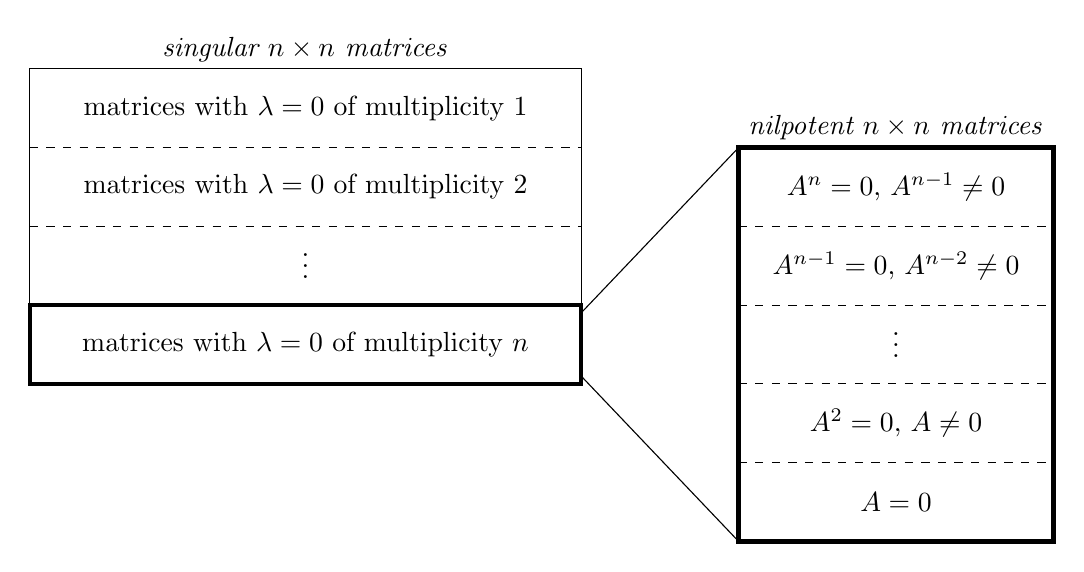
\begin{tikzpicture}

\node at (3.5,4.25) {\textit{singular $n \times n$ matrices}};
\draw (0,4) to (7,4);
\node at (3.5,3.5) {matrices with $\lambda = 0$ of multiplicity $1$};
\draw[dashed] (0,3) to (7,3);
\node at (3.5,2.5) {matrices with $\lambda = 0$ of multiplicity $2$};
\draw[dashed] (0,2) to (7,2);
\node at (3.5,1.6) {$\vdots$};
\draw[dashed] (0,1) to (7,1);
\node at (3.5,0.5) {matrices with $\lambda = 0$ of multiplicity $n$};
\draw (0,0) to (7,0) to (7,4) to (0,4) to cycle;

\draw[ultra thick] (0,0) to (7,0) to (7,1) to (0,1) to cycle;
\begin{scope}[xshift=9cm,yshift=-2cm]
	\node at (2,5.25) {\textit{nilpotent $n \times n$ matrices}};
	\node at (2,4.5) {$A^n = 0$, $A^{n-1} \neq 0$};
	\draw[dashed] (0,4) to (4,4);
	\node at (2,3.5) {$A^{n-1} = 0$, $A^{n-2} \neq 0$};
	\draw[dashed] (0,3) to (4,3);
	\node at (2,2.6) {$\vdots$};
	\draw[dashed] (0,2) to (4,2);
	\node at (2,1.5) {$A^2 = 0$, $A \neq 0$};
	\draw[dashed] (0,1) to (4,1);
	\node at (2,0.5) {$A = 0$};
	\draw[ultra thick] (0,0) to (4,0) to (4,5) to (0,5) to cycle;
\end{scope}

\draw (7,0.9) to (9,3);
\draw (7,0.1) to (9,-2);

\end{tikzpicture}
